% COMS 6998, Fall 2026 -- P3: Evaluation Plan & Initial Results
% Course template (IEEEtran, two pages excluding references). Build: latexmk -pdf main.tex
%
% HOW THIS SKELETON WORKS
%   \pw{...}   = a slot for your own prose (prints in red so nothing is left behind).
%   % FACTS:   = numbers and pointers you can use in that slot, all from the repo.
%   Tables and figures hold real data from results/2026-11-19-space-multitenancy-initial
%   (12 frames per cell). Captions are left as slots too.
%   Delete the FACTS comments and \pw macros before submitting.

\documentclass[conference,10pt,letterpaper]{IEEEtran}
\usepackage[T1]{fontenc}
\usepackage{cite}
\usepackage{graphicx}
\usepackage{booktabs}
\usepackage{tabularx}
\usepackage{xcolor}
\usepackage{flushend}
\usepackage[hyphens]{url}
\usepackage[hidelinks]{hyperref}

\newcommand{\pw}[1]{\textcolor{red}{\textit{[#1]}}}

% Same title as P2; change it if the multi-tenancy angle is now the main claim.
\title{Where Edge Inference Misses Its Deadline:\\Latency Tails on a Shared Jetson Thor}
\author{\IEEEauthorblockN{Pulak Mehrotra (pm3371)}
\IEEEauthorblockA{COMS 6998: AI-Native Computing $\mid$ Fall 2026\\
P3: Evaluation Plan \& Initial Results $\mid$ Due November 25, 2026, 11:59 PM ET}}

\begin{document}
\maketitle
\thispagestyle{plain}
\pagestyle{plain}

% =====================================================================
\section{Project Goal and Updates}
% Template asks: goal, research question, the main claim you will test,
% and what changed since P2 (incl. midterm + P2 feedback) and why.

\textbf{Goal.} \pw{goal and research question(s), carried over from P2's Q1/Q2}
% FACTS (P2): Q1 how often does inference miss a per-input deadline?
%   Q2 how much of each miss comes from the model vs co-located GPU work,
%   frequency scaling, host-side overhead?

\textbf{Claim.} \pw{the one claim this report tests}
% FACTS: P2 already concluded "the model is not the source of variance; sharing is"
%   (alone prefill p99/p50 = 1.005). A natural P3 claim is about HOW the GPU is
%   shared: time-slicing gives a frame time of about alone x (1 + busy neighbours),
%   MPS partitions are predictable but slow all the time.

\textbf{Updates since P2.} \pw{what changed and why}
% FACTS (things that changed, so you can pick what to explain):
%   - Focus moved from "one co-tenant we don't control" to controlled
%     multi-tenancy: other VLM tenants, each in its own container, sharing by
%     time-slicing or by static MPS partitions (branch space-multitenancy-v1).
%   - P2 next steps NOT yet done: alone cells at T = 20/5/2/1.5 s (gate 3),
%     light/heavy/memcpy co-runners (gate 4), clock-pinned idle-gap test.
%     Zishen will notice if these vanish silently -- say where they went.
%   - P2's main risk is gone: we now have sudo (nvpmodel, jetson_clocks, ncu)
%     and labmates coordinate, so no GPU booking (TODO.md, 2026-11-19).
%   - Fixed since P2: feeder now logs scheduled arrival; frame counts split into
%     served / overwritten / error; probe no longer runs a 4-token decode before
%     each timed request (the gate-2 spread was measured that way).
%   - Midterm feedback: \pw{fill in}

% =====================================================================
\section{Evaluation Setup}
% Template asks: workloads (incl. >=1 held-out workload/config/scale),
% >=2 baselines (a classical/non-agentic one where applicable), metrics
% (task quality + systems metrics), platform. Table or paragraphs, your call.

\textbf{Platform.} \pw{platform}
% FACTS: Jetson AGX Thor, JetPack 7, CUDA 13.2, 122 GB unified memory, 20 SMs,
%   120 W mode. llama.cpp llama-server built for sm_110, single slot.
%   Each tenant in its own container (container smoke test: same speed as host,
%   1.52 s back to back). Private MPS daemon so labmates cannot join it.
%   Initial cells had the GPU clock NOT pinned; final cells: sudo jetson_clocks.

\textbf{Workloads.} \pw{workloads, and which one is held out}
% FACTS: Stack A = Gemma 3 4B QAT Q4_0, 896x896 Sentinel-2 tiles, keep/drop in
%   one token (301 prompt tokens). Measured tenant 0 gets a tile every T s.
%   Neighbours run the same model: bursty (bursts of 5, one burst per ~15 s,
%   random start) or saturating (next request as soon as the last returns);
%   planned: steady. Tenants: 1, 3 done; 2 and 5 planned (split 20 SMs exactly).
%   Held-out candidates: (a) 2 and 5 tenants, (b) T = 3 s where the mailbox
%   overwrites frames, (c) Stack B: SmolVLA / pi0.5 with an action-chunk deadline.

\textbf{Baselines.} \pw{baselines and what each represents}
% FACTS: this is a measurement study, so the "baselines" are ways of sharing:
%   (1) alone on the GPU (the lower bound),
%   (2) default time-slicing (what you get with no configuration),
%   (3) static MPS partitions (equal SMs per tenant, 2-SM granularity),
%   planned (4) MPS without partitions.

\textbf{Metrics.} \pw{metrics}
% FACTS: deadline-miss rate at any D (applied offline; latency = t_end - t_obs,
%   overwritten frame = miss), p50 / p99, energy per frame from the 100 Hz power
%   trace. Task quality: keep/drop agreement with SCL ground truth, 48/50 = 96%
%   (gate 2); sharing does not change the answer, only when it arrives.
%   With 12 frames a miss rate has a ~+-25 point 95% interval; 60 frames planned.

% =====================================================================
\section{Initial Results}
% Template asks: >=1 figure or table stating workload, baselines, metrics,
% configuration and number of runs; what it suggests; does it support the
% claim; anything that surprised you.

\begin{table}[t]
\caption{\pw{caption}}
\label{tab:tenancy}
\centering
\small
\begin{tabular}{@{}llrrr@{}}
\toprule
Neighbours & Sharing & p50 (s) & p99 (s) & Miss @ 3\,s \\
\midrule
none (alone)  & --             & 1.55 & 1.56 & 0/12 \\
bursty        & time-slicing   & 2.98 & 4.01 & 6/12 \\
bursty        & MPS partitions & 4.43 & 4.47 & 12/12 \\
saturating    & time-slicing   & 4.54 & 4.73 & 12/12 \\
saturating    & MPS partitions & 4.45 & 4.52 & 12/12 \\
\bottomrule
\end{tabular}
\end{table}
% Table source: results/2026-11-19-space-multitenancy-initial (README table;
% p50 and miss counts rechecked from requests.csv). One run per cell, 12 frames,
% T = 6 s (no queueing), 3 tenants, MPS = 6 SMs each with 2 SMs idle.

\begin{figure*}[t]
\centering
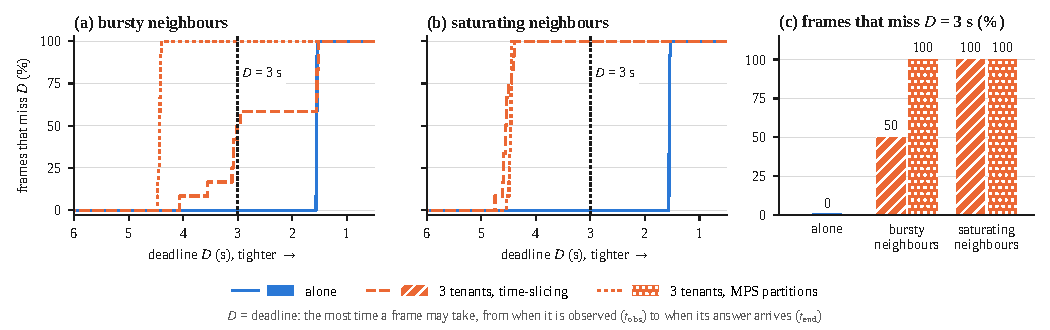
\includegraphics[width=\textwidth]{figures/miss_rate_timeslice_vs_mps.pdf}
\caption{\pw{caption}}
\label{fig:miss}
\end{figure*}
% Alternative figure (shows WHY time-slicing is poor, frame by frame):
%   figures/timeline_bursty.pdf (7.0 x 2.95 in, taller). Two pages is tight,
%   so probably one figure* + Table I. figures/p99_timeslice_vs_mps.pdf also exists.

\pw{what the table and figure say}
% FACTS (results README):
%   - Alone 1.55 s. Two busy neighbours: ~4.5 s under either sharing, 2.9x
%     slower, close to the 3x fair time-slicing predicts.
%   - Time-slicing: frame ~ alone x (1 + busy neighbours). One busy neighbour
%     = 3.06 s, so a 3 s deadline can't absorb even one. Bursty neighbours only
%     38% busy still made 6/12 frames miss (1.5 s outside a burst, 3-4 s inside).
%   - MPS partitions isolate: 4.43 vs 4.45 s whatever the neighbours do, tighter
%     tail (p99 4.52 vs 4.73 s), but slow even when neighbours are idle.

\pw{does this support the claim; what surprised you}
% FACTS: surprise candidates -- 6 of 20 SMs is about as slow as a 3-way share of
%   all 20 (why = issue #14); MPS wasn't faster on average at all.
%   Caveats to state: 12 frames, clock not pinned (alone cell started frames at
%   315 MHz), ~80 s cells so a bursty neighbour fired only 1-5 bursts and load
%   differs between cells.
% Optional pilot (S6, no results folder yet): flash attention on vs off,
%   1.55 s -> 1.17 s per frame. Check the numbers before using.

% =====================================================================
\section{Planned Ablations and Next Steps}
% Template asks: each ablation = what you remove/vary, which part of the claim
% it tests, expected outcome; one failure/boundary case; plan for M4 (Dec 7):
% main results, >=1 ablation, a failure/boundary case, repeated measurements.

\pw{ablations: what you vary, what it tests, what you expect}
% FACTS (issue #20 experiment tracker; pick what fits by Dec 7):
%   S3 full matrix: 1/2/5 tenants x steady/bursty/saturating x time-slicing /
%      MPS / MPS partitions, 60 frames, clock pinned, achieved neighbour load logged.
%   S5 why partitions cost what they cost: alone on 10 / 6 / 4 SM partitions,
%      nsys of one time-sliced and one partitioned cell (#14).
%   S7 bandwidth-only co-runner: EdgePace found bandwidth, not compute, hurts on
%      unified memory -- separates SM contention from memory contention.
%   P2 clock pinned vs not, for the idle-gap slowdown (SmolVLA 1.54x at 1 Hz).
%   S8 a lower power mode (now possible with sudo).

\pw{failure or boundary case}
% FACTS: S4 -- T = 3 s, where a slow frame also delays/overwrites the next one
%   through the mailbox (cascading misses). Or: the tenant count where even
%   partitions can't meet D.

\pw{Milestone 4 plan (Dec 7) and how you'll handle repeats/uncertainty}
% FACTS: 60-frame cells -> ~+-12 points on a miss rate; Wilson CIs already in the
%   reporter; repeat each cell \pw{N} times.

% Uncomment once something is cited (an empty bibliography is a LaTeX error).
% Keys in references.bib: earthplus, naviorbital, jetsonpi, gemma3, pi05, mps.
% \bibliographystyle{IEEEtran}
% \bibliography{references}

\end{document}
